\documentclass[10pt, titlepage]{article}

\usepackage[margin=1in]{geometry}
\usepackage{graphicx}
\usepackage{float}
\usepackage{xcolor,listings}
\usepackage[most]{tcolorbox}
\usepackage{times} % for Times New Roman font
\usepackage{setspace} % for single spacing
\parindent 0px % no indentation

\title{\textbf{ECCS 3411\\Computer Security}\\Midterm Project Report}
\author{Kento Akazawa, Grant Daly, Brian Watkins}
\date{April 28, 2024}

\lstdefinelanguage{swift}
{
  morekeywords={
    func,if,then,else,for,in,while,do,switch,case,default,where,break,continue,fallthrough,return,
    typealias,struct,class,enum,protocol,var,func,let,get,set,willSet,didSet,inout,init,deinit,extension,
    subscript,prefix,operator,infix,postfix,precedence,associativity,left,right,none,convenience,dynamic,
    final,lazy,mutating,nonmutating,optional,override,required,static,unowned,safe,weak,internal,
    private,public,is,as,self,unsafe,dynamicType,true,false,nil,Type,Protocol,VStack,HStack,Text
  },
  morecomment=[l]{//}, % l is for line comment
  morecomment=[s]{/*}{*/}, % s is for start and end delimiter
  morestring=[b]" % defines that strings are enclosed in double quotes
}

\definecolor{keyword}{HTML}{BA2CA3}
\definecolor{string}{HTML}{D12F1B}
\definecolor{comment}{HTML}{008400}
\definecolor{lightgray}{HTML}{F5F5F5}

\lstset{
  language=swift,
  basicstyle=\ttfamily,
  showstringspaces=false, % lets spaces in strings appear as real spaces
  columns=fixed,
  keepspaces=true,
  numbers=left,
  numberstyle=\tiny\color{gray},
  showstringspaces=false,
  keywordstyle=\color{keyword},
  stringstyle=\color{string},
  commentstyle=\color{comment},
  backgroundcolor=\color{lightgray},
  linewidth=0.95\textwidth
}

\begin{document}
\maketitle
\newpage

\section*{Introduction}
In today's digital landscape, where online security is paramount, the need for robust password management solutions has never been greater. For this project, we created password manager app in Swift. It offers users a secure and convenient way to store their passwords, along with associate usernames and titles. Leveraging advanced encryption and hashing techniques, this app ensures that sensitive user data remains protected against unauthorized access and potential breaches.

\section*{Data}
Access to stored passwords is controlled by a master password, ensuring confidentiality. Each password entry is assigned a unique ID, allowing for efficient management of multiple entries with the same title and username. Leveraging \texttt{CoreData}, passwords are stored securely within the application's database. 

\section*{UI}
When launching the app for the first time, it asks to set the master password as shown in Figure \ref{fig:set_pw} below. 
\begin{figure}[H]
	\centering
	\vspace{-0.25em}
	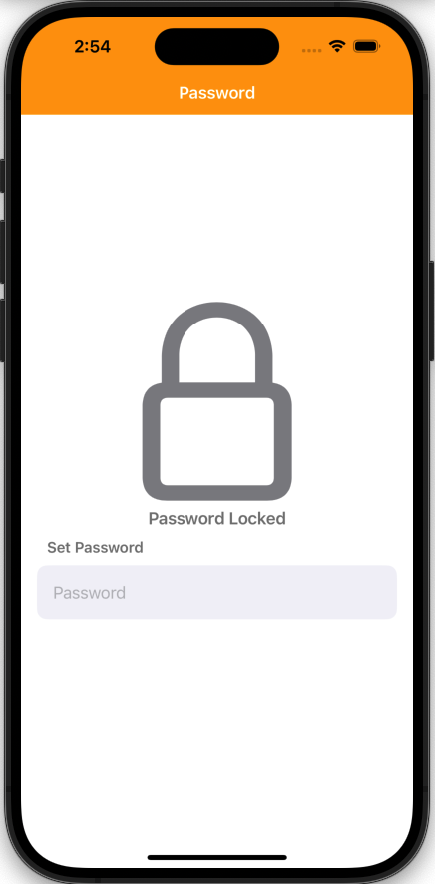
\includegraphics[width=0.4\textwidth]{img/set_pw}
	\vspace{-0.75em}
	\caption{Setting Master Password}
	\label{fig:set_pw}
	\vspace{-0.75em}
\end{figure}

Enhancing the security of our application, we implement a robust measure by hashing the master password using the SHA-256 algorithm before storage. This one-way hashing process ensures that even in the event of a breach, the original password remains secure since it is computationally infeasible to determine it from hashed password. The code for hashing the master password is shown below. 
\begin{center}
\begin{minipage}{\textwidth}
\begin{lstlisting}
private func hashPassword(_ pw: String) -> String {
  guard let passwordData = pw.data(using: .utf8) else {
    fatalError("Failed to convert password to data")
  }

  // hash the password using SHA-256
  // and convert to hexadecimal string
  return SHA256.hash(data: passwordData).map
    { String(format: "%02x", $0) }.joined()
}
\end{lstlisting}
\end{minipage}
\end{center}

The function take a password string \texttt{pw} as input and returns its SHA-256 hash as a hexadecimal string. First, the password string is converted into data using UTF-8 encoding. Next, the SHA-256 hash is computed using \texttt{SHA256.hash(data:)} function from \texttt{CryptoKit} framework. The resulting hash is then mapped to a string array, with each byte of the hash being converted into its hexadecimal representation. This hexadecimal representation is joined into a single string, which is returned as the output of the function. 

When the app launches after the master password is set, it asks for the password as shown in Figure \ref{fig:enter_pw}.
\begin{figure}[H]
	\centering
	\vspace{-0.25em}
	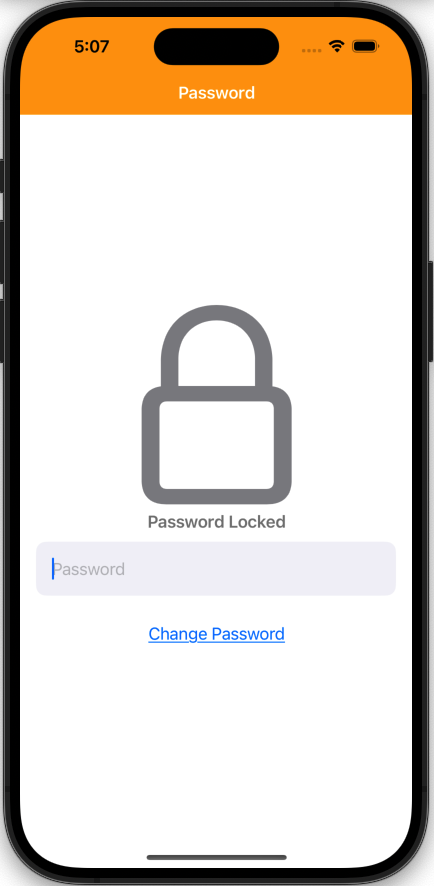
\includegraphics[width=0.3\textwidth]{img/enter_pw}
	\vspace{-0.75em}
	\caption{Entering Password}
	\label{fig:enter_pw}
	\vspace{-0.75em}
\end{figure}

The entered password will be hashed and compared with saved hashed master password. The function that checks if entered password is correct is shown below.
\begin{center}
\begin{minipage}{\linewidth}
\begin{lstlisting}
func doesMasterPasswordMatch(_ pw: String) -> Bool {
  guard let masterPw = UserDefaults.standard.string(forKey: masterPwKey)
  else { return false }
  return hashPassword(pw) == masterPw
}
\end{lstlisting}
\end{minipage}
\end{center}
The function retrieves the hashed master password stored locally on the device using \texttt{UserDefaults.standard.} \texttt{string(forKey: masterPwKey)}. Next, it calculates the hash of entered password and compares with saved password. If they do not match, it displays a message showing that entered password is wrong as shown in Figure \ref{fig:enter_wrong_pw}. 
\begin{figure}[H]
	\centering
	\vspace{-0.25em}
	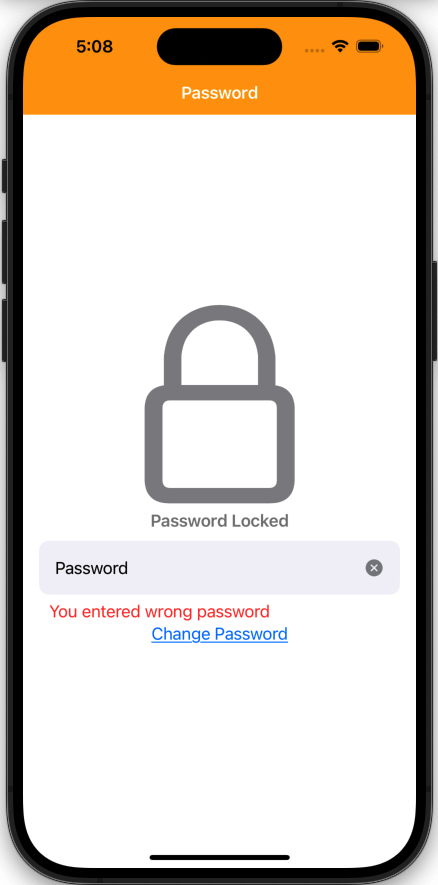
\includegraphics[width=0.3\textwidth]{img/enter_wrong_pw}
	\vspace{-0.75em}
	\caption{When wrong password is entered}
	\label{fig:enter_wrong_pw}
	\vspace{-0.75em}
\end{figure}

Password can be changed by tapping \texttt{Change Password} link. This navigates to a screen shown in Figure \ref{fig:change_pw}.
\begin{figure}[H]
	\centering
	\vspace{-0.25em}
	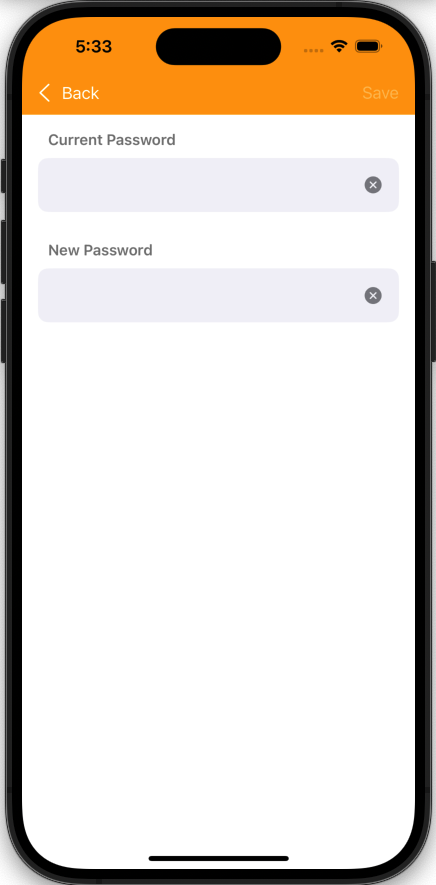
\includegraphics[width=0.3\textwidth]{img/change_pw}
	\vspace{-0.75em}
	\caption{Changing master password}
	\label{fig:change_pw}
	\vspace{-0.75em}
\end{figure}
Once current password and new password are entered, save button on the top right will be enabled. If the current password matches with the saved password, new master password will be saved and navigate back to the initial screen (Figure \ref{fig:enter_pw}).

If the entered password is correct in the initial screen (Figure \ref{fig:enter_pw}), it grants access to the list of passwords saved and displays them as shown in Figure \ref{fig:pw_list}.
\begin{figure}[H]
	\centering
	\vspace{-0.25em}
	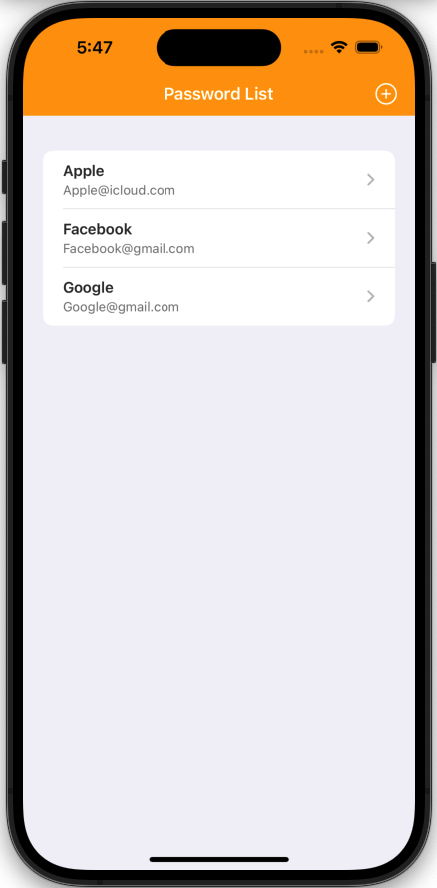
\includegraphics[width=0.3\textwidth]{img/pw_list}
	\vspace{-0.75em}
	\caption{List of saved passwords}
	\label{fig:pw_list}
	\vspace{-0.75em}
\end{figure}
New password can be added by tapping on plus symbol on the top right. It will navigate to screen shown in Figure \ref{fig:add_pw}.
\begin{figure}[H]
	\centering
	\vspace{-0.25em}
	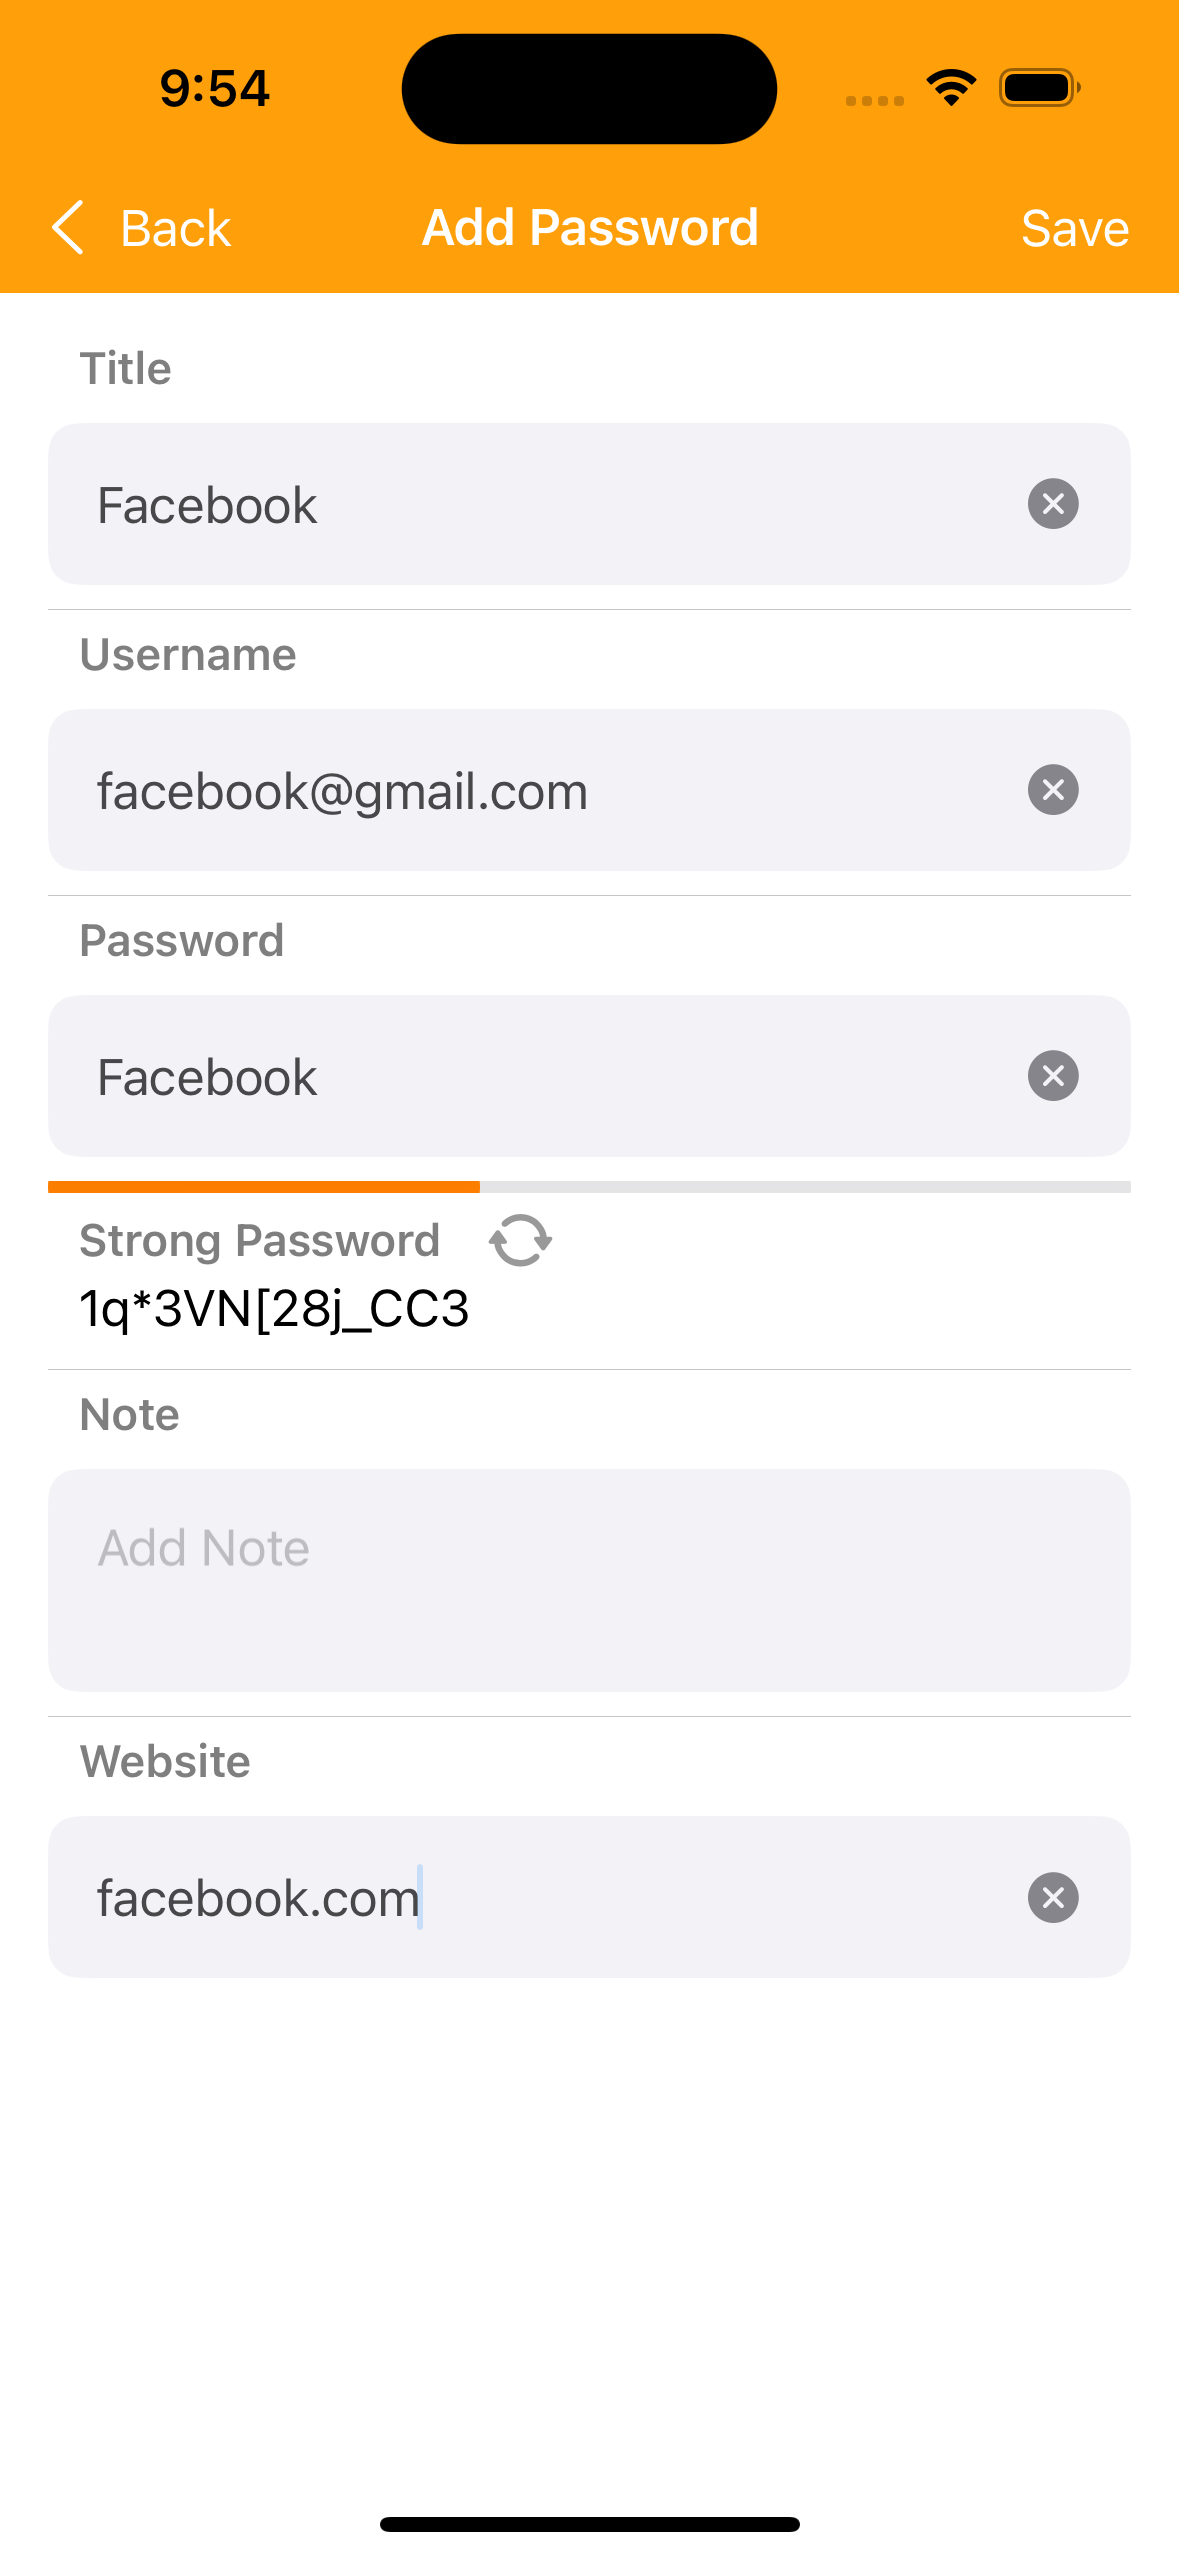
\includegraphics[width=0.3\textwidth]{img/add_pw}
	\vspace{-0.75em}
	\caption{Adding new password}
	\label{fig:add_pw}
	\vspace{-0.75em}
\end{figure}

Each stored password comprises a title, username, and password. When users access the password list screeen (Figure \ref{fig:pw_list}), they are presented with the titles and usernames of their stored passwords. Upon selecting a specific entry, users are directed to the password detail screen (Figure \ref{fig:pw_detail_0}), where the password is initially concealed to protect against shoulder surfing. However, users can reveal the password by tapping on it, as depicted in Figure \ref{fig:pw_detail_1}. This approach balances security with usability, allowing users quick access to their passwords while maintaining confidentiality.
\begin{figure}[H]
	\centering
	\vspace{-0.25em}
	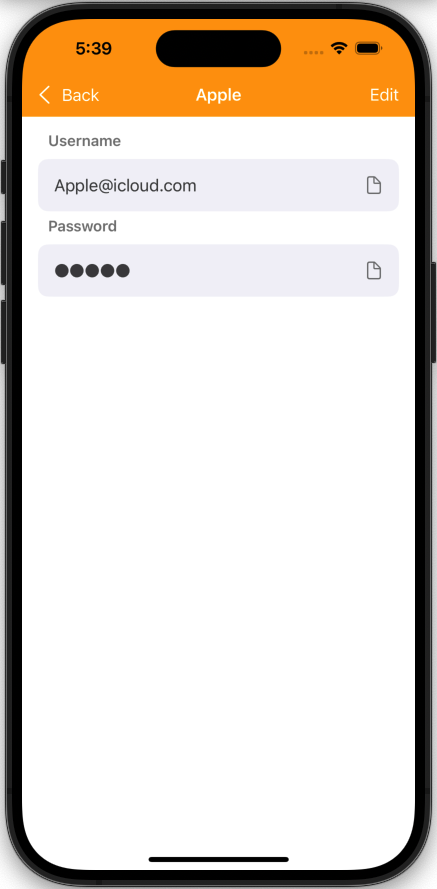
\includegraphics[width=0.3\textwidth]{img/pw_detail_0}
	\vspace{-0.75em}
	\caption{Password detail view}
	\label{fig:pw_detail_0}
	\vspace{-0.75em}
\end{figure}

\begin{figure}[H]
	\centering
	\vspace{-0.25em}
	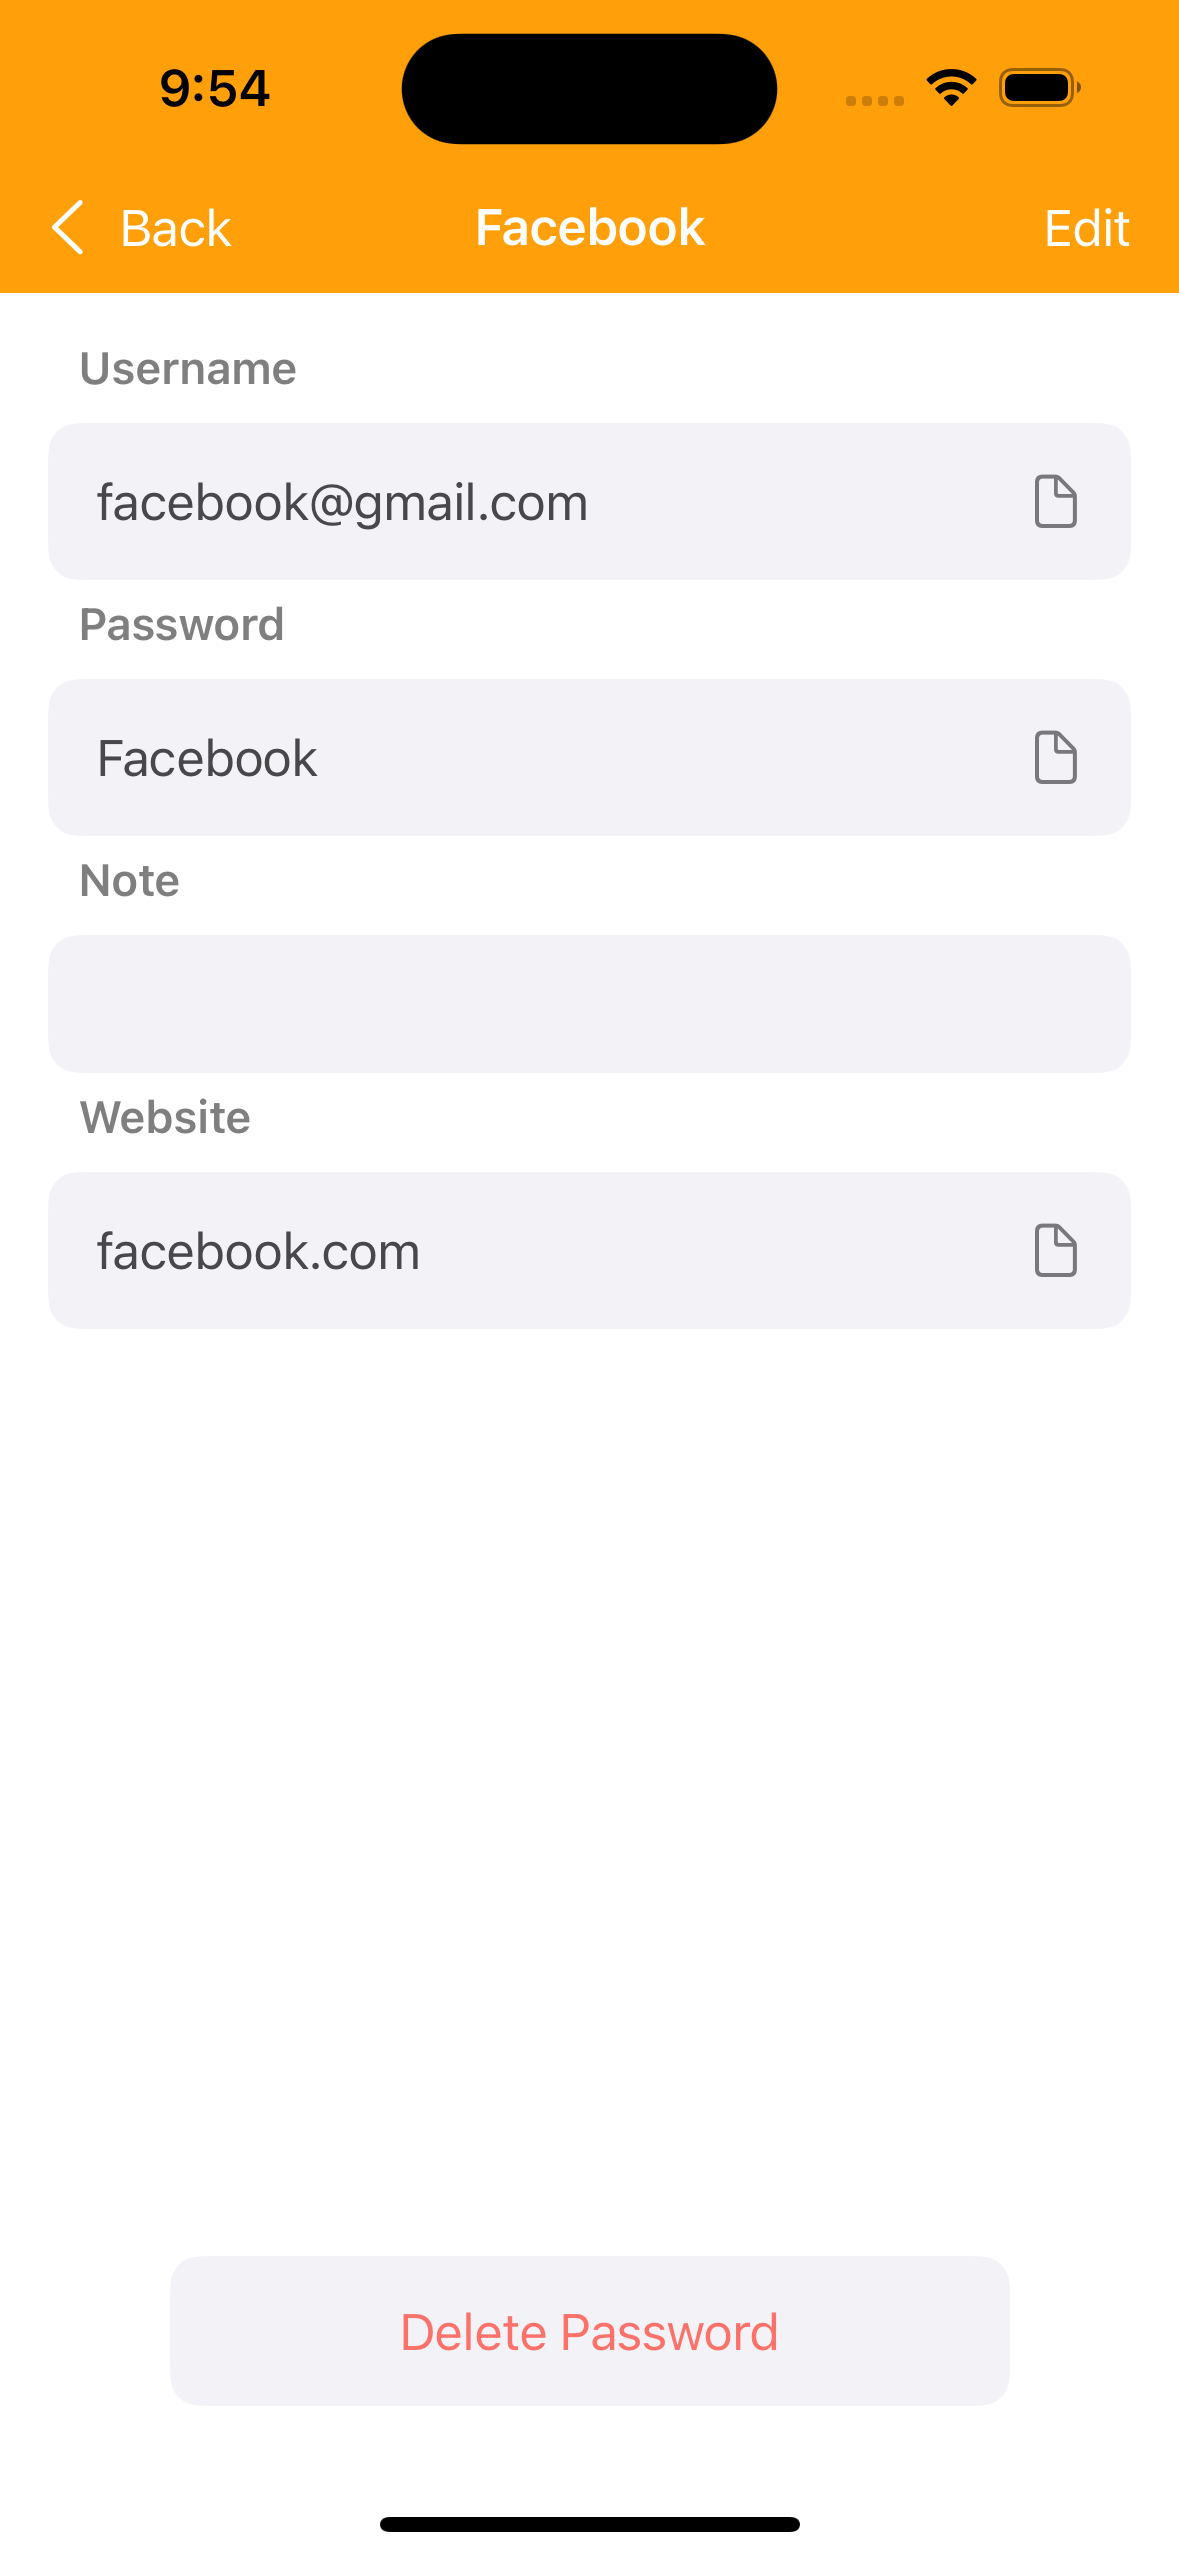
\includegraphics[width=0.3\textwidth]{img/pw_detail_1}
	\vspace{-0.75em}
	\caption{Password detail view}
	\label{fig:pw_detail_1}
	\vspace{-0.75em}
\end{figure}

\section*{Encryption}
In our password manager app, security is paramount. Every password is encrypted using the Advanced Encryption Standard (AES) with Galois Counter Mode (GCM), a highly secure encryption method endorsed by prestigious organizations worldwide. AES has become the encryption standard of choice, endorsed by the US Government and numerous prestigious organizations worldwide \cite{team_password}. Hackers can only crack an AES-encrypted password by employing a brute-force attack, attempting various password combinations until they find the correct one. AES-GCM operates with a symmetric key, meaning the same key is used for both encryption and decryption processes. This symmetric key system ensures efficiency and security, as it simplifies the encryption and decryption processes while maintaining robust protection against unauthorized access. 
\begin{center}
\begin{minipage}{\linewidth}
\begin{lstlisting}
private let symmetricKey = "Symmetric Key"
private var key = SymmetricKey(size: .bits256)

init() {
  if let keyData = UserDefaults.standard.data(forKey: symmetricKey) {
    do {
      key = try SymmetricKey(data: keyData)
    } catch {
    // error initializing symmetric key from data
    print("Error initializing SymmetricKey from data:", error)
    }
  } else {
    // generate symmetric key if it doesn't exist yet
    key = SymmetricKey(size: .bits256)
    do {
      // convert symmetric key to Data and store in UserDefaults
      let keyData = try key.withUnsafeBytes { Data($0) }
      UserDefaults.standard.set(keyData, forKey: symmetricKey)
    } catch {
      // error converting symmetric key to data
      print("Error converting SymmetricKey to data:", error)
    }
  }
}
\end{lstlisting}
\end{minipage}
\end{center}
It begins by defining constant \texttt{symmetricKey} to hold the identifier for storing and retrieving the key from user defaults and initializing symmetric key using \texttt{SymmetricKey(size: .bits256)} which creates a symmetric key with 256 bits. 

Within the \texttt{init()} method, it attempts to retrieve the symmetric key stored in the user defaults under the identifier \texttt{symmetricKey}. If the key data is found, it is used to initialize \texttt{key} variable. Otherwise, key has not been generated yet, so a new symmetric key of size 256 bits will be generated. This newly generated key is then converted into a \texttt{Data} object and stored in the user defaults under the \texttt{symmetricKey} identifier for future use. When adding a new password or changing existing password, this \texttt{key} is used to encrypt.

\begin{center}
\begin{minipage}{\linewidth}
\begin{lstlisting}
func addPassword(_ pw: Password, context: NSManagedObjectContext) {
  guard let password = encrypt(pw.password) else { return }
  DataController().addPassword(title: pw.title, 
                               username: pw.username,
                               password: password,
                               context: context)
}

func editPassword(_ pw: Password, to passwords: Passwords, 
                    context: NSManagedObjectContext) {
  guard let password = encrypt(pw.password) else { return }
  DataController().editPassword(passwords, 
                                title: pw.title,
                                username: pw.username,
                                password: password,
                                context: context)
}
\end{lstlisting}
\end{minipage}
\end{center}
When adding or editing the password, password is encrypted before storage. This process ensures that sensitive user information remains protected against unauthorized access. The code for encryption is shown below. 
\begin{center}
\begin{minipage}{\linewidth}
\begin{lstlisting}
private func encrypt(_ pw: String) -> Data? {
  guard let data = pw.data(using: .utf8) else { return nil }
  do {
    let sealedBox = try AES.GCM.seal(data, using: key)
    return sealedBox.combined
  } catch {
    print("Encryption failed: \(error.localizedDescription)")
    return nil
  }
}
\end{lstlisting}
\end{minipage}
\end{center}
The encryption process begins by converting the plaintext password into a \texttt{Data} object using UTF-8 encoding. This step ensures that the password is in a format suitable for cryptographic operations. Next, the function utilizes the AES-GCM to perform the encryption. 

Within a do-catch block, the encryption attempts to use the \texttt{AES.GCM.seal} method, which seals the plaintext data using the provided encryption key, \texttt{key}. If successful, the encrypted data is encapsulated within a sealed box. Finally, the combined ciphertext and authentication tag are extracted from the sealed box and returned as Data.

\begin{center}
\begin{minipage}{\linewidth}
\begin{lstlisting}
func getPassword(_ encryptedData: Data) -> String {
  guard let pw = decryptPassword(encryptedData) else { return "" }
  return pw
}

private func decryptPassword(_ encryptedData: Data) -> String? {
  do {
    let sealedBox = try AES.GCM.SealedBox(combined: encryptedData)
    let decryptedData = try AES.GCM.open(sealedBox, using: key)
    return String(data: decryptedData, encoding: .utf8)
  } catch {
    print("Decryption failed: \(error.localizedDescription)")
    return nil
  }
}
\end{lstlisting}
\end{minipage}
\end{center}
When displaying the password, the program needs to decrypt the saved password. The function, \texttt{decryptPassword} uses same symmetric key to decrypt. The encrypted data is first encapsulated within a sealed box using the AES-GCM algorithm. This sealed box is then passed to the \texttt{AES.GCM.open} method along with the symmetric key. If successful, the decrypted data is obtained, and it is converted back to a string using UTF-8 encoding.

\begin{center}
\begin{minipage}{\linewidth}
\begin{lstlisting}
\end{lstlisting}
\end{minipage}
\end{center}

\section*{Conclusion}
The password manager app developed in Swift ensures robust security for managing passwords. It employs advanced encryption and hashing techniques, including SHA-256 for hashing master password and AES-GCM algorithm for encrypting and decrypting passwords. By prioritizing both security and convenience, the app addresses the crucial need for safeguarding sensitive data.

\newpage
\bibliographystyle{IEEEtran}
\bibliography{references}

\end{document}